\documentclass[8pt,a4paper,compress]{beamer}

\usepackage{/home/siyer/lib/slides}

\title{Balanced Search Trees}
\date{}

\begin{document}
\begin{frame}
\vfill
\titlepage
\end{frame}

\section{2-3 Search Trees}
\begin{frame}[fragile]
\pause

A 2-3 search tree is a tree that is either empty (null link) or
\begin{itemize}
\pause
\item A 2-node with one key (and associated value) and two links, a left link to a 2-3 search tree with smaller keys, and a right link to a 2-3 search tree with larger keys

\pause
\item A 3-node with two keys (and associated values) and three links, a left link to a 2-3 search tree with smaller keys, a middle link to a 2-3 search tree with keys between the node's keys, and a right link to a 2-3 search tree with larger keys
\end{itemize}

\pause
\begin{center}
\visible<5->{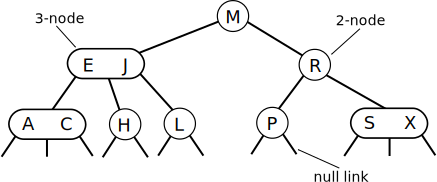
\includegraphics[scale=0.4]{{./figures/23_tree}.pdf}}
\end{center}

\pause
\bigskip

A 2-3 search tree has symmetric order --- inorder traversal yields keys in ascending order

\pause
\bigskip

A perfectly balanced 2-3 search tree is one whose null links are all the same distance from the root

\begin{center}
\visible<7->{\includegraphics[scale=0.3]{{./figures/23_tree_perfect_balance}.png}}
\end{center}
\end{frame}

\begin{frame}[fragile]
\pause

Searching for a key in a 2-3 tree
\begin{center}
\visible<3->{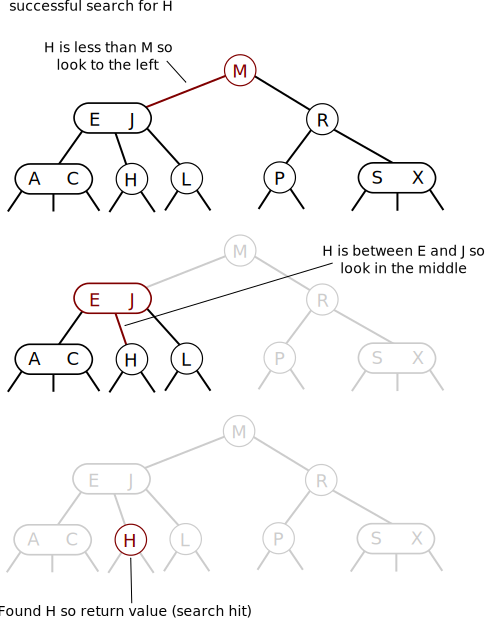
\includegraphics[scale=0.37]{{./figures/23_tree_search1}.pdf}}\hfill
\visible<4->{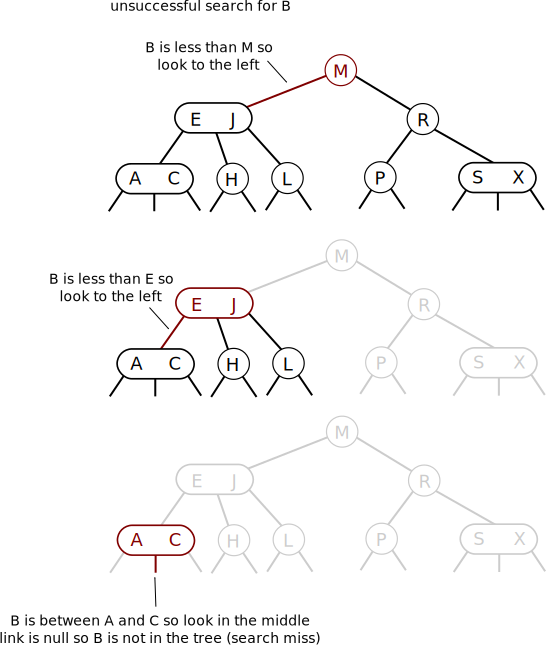
\includegraphics[scale=0.37]{{./figures/23_tree_search2}.pdf}}
\end{center}
\end{frame}

\begin{frame}[fragile]
\pause

Inserting a key into a 2-node

\begin{center}
\visible<2->{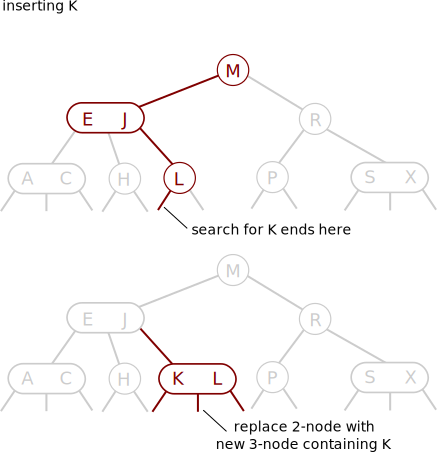
\includegraphics[scale=0.5]{{./figures/23_tree_insert1}.pdf}}
\end{center}
\end{frame}

\begin{frame}[fragile]
\pause

Inserting a key into a single 3-node
\begin{center}
\visible<2->{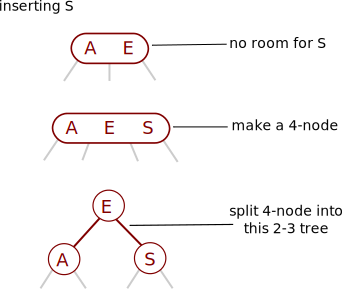
\includegraphics[scale=0.5]{{./figures/23_tree_insert2}.pdf}}
\end{center}
\end{frame}

\begin{frame}[fragile]
\pause

Inserting a key into a 3-node whose parent is a 2-node
\begin{center}
\visible<2->{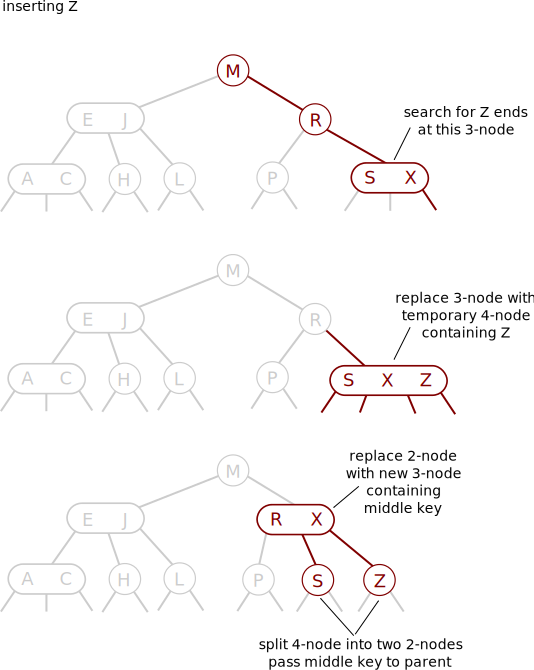
\includegraphics[scale=0.4]{{./figures/23_tree_insert3}.pdf}}
\end{center}
\end{frame}

\begin{frame}[fragile]
\pause

Inserting a key into a 3-node whose parent is a 3-node
\begin{center}
\visible<2->{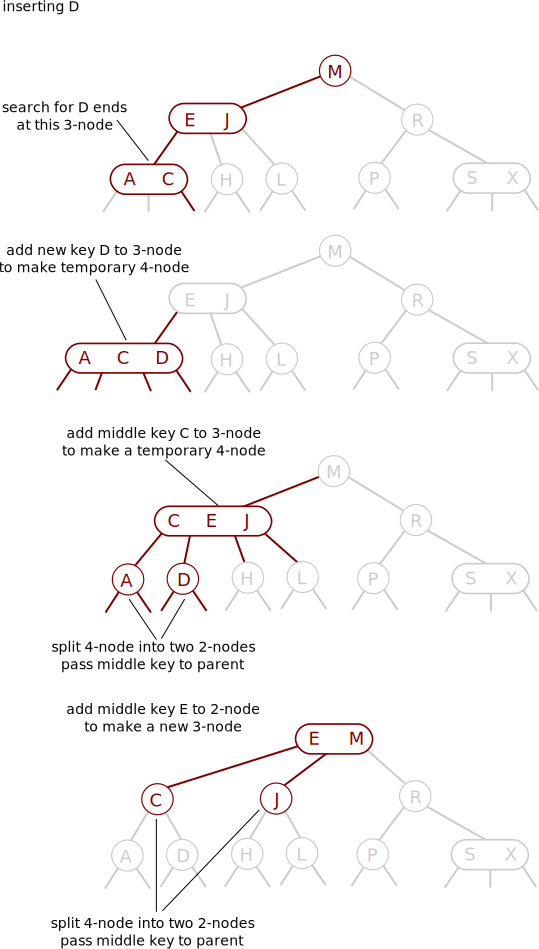
\includegraphics[scale=0.3]{{./figures/23_tree_insert4}.pdf}}
\end{center}
\end{frame}

\begin{frame}[fragile]
\pause

Splitting the root
\begin{center}
\visible<2->{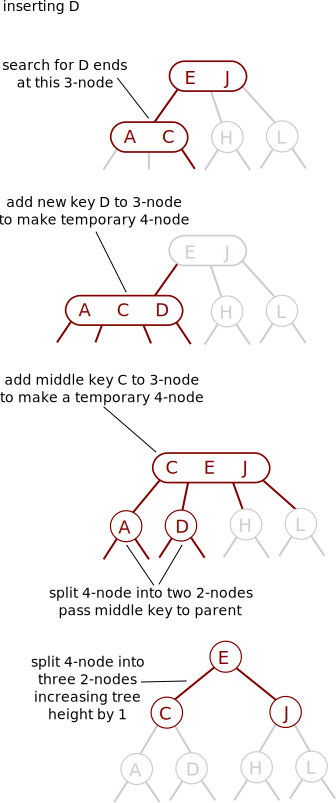
\includegraphics[scale=0.33]{{./figures/23_tree_insert5}.pdf}}
\end{center}
\end{frame}

\begin{frame}[fragile]
\pause

Splitting a 4-node is a local transformation, and thus involves constant number of operations

\pause
\bigskip

Insert operation maintains symmetric order and perfect balance

\pause
\bigskip

Tree height
\begin{itemize}
\pause
\item Worst case: $\lg N$ (all 2-nodes)
\pause
\item Best case: $\log_3 N \approx 0.631 \lg N$ (all 3-nodes)
\pause
\item Between 12 and 20 for a million nodes
\pause
\item Between 18 and 30 for a billion nodes
\end{itemize}

\pause
\bigskip

Guaranteed logarithmic performance for search and insert
\end{frame}

\section{Red-Black BSTs}
\begin{frame}[fragile]
\pause

We represent a 2-3 tree as a BST, using ``internal'' left-leaning links as ``glue'' for 3-nodes

\begin{center}
\visible<2->{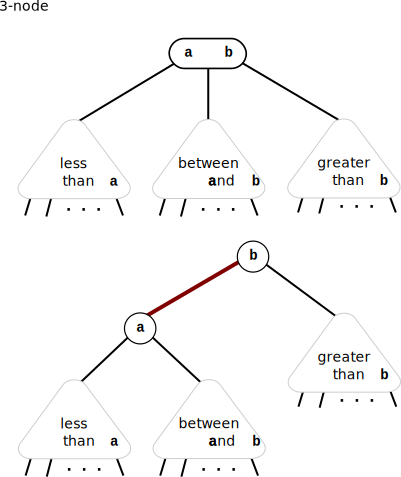
\includegraphics[scale=0.5]{{./figures/red_black_bst1}.pdf}}
\end{center}
\end{frame}

\begin{frame}[fragile]
\pause

A red-black tree is a BST such that
\begin{itemize}
\pause
\item No node has two red links connected to it
\pause
\item Every path from root to null link has the same number of black links (perfect black balance)
\pause
\item Red links lean left
\end{itemize}

\begin{center}
\visible<6->{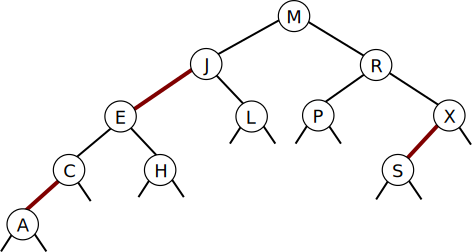
\includegraphics[scale=0.5]{{./figures/red_black_bst2}.pdf}}
\end{center}
\end{frame}

\begin{frame}[fragile]
\pause

One-to-one correspondence between red-black BSTs and 2-3 trees

\begin{center}
\visible<2->{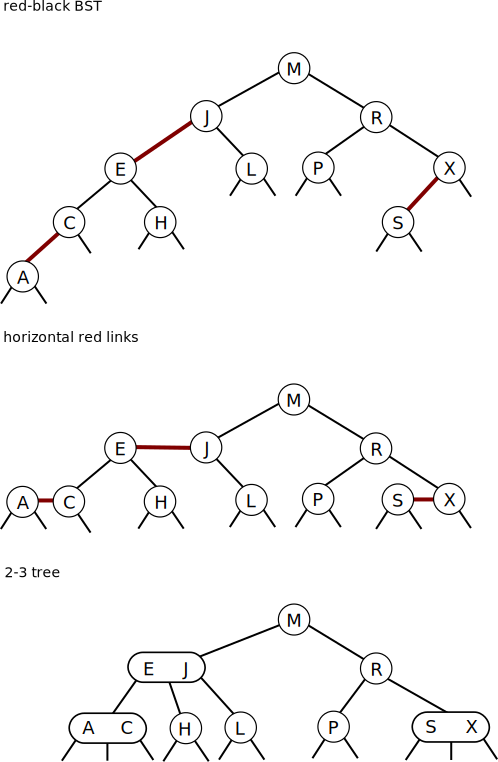
\includegraphics[scale=0.35]{{./figures/red_black_bst3}.pdf}}
\end{center}
\end{frame}

\begin{frame}[fragile]
\pause

Red-black BST representation: each node is pointed to by precisely one link (from its parent) $\implies$ can encode color of links in nodes

\begin{minipage}{170pt}
\begin{lstlisting}[language=Java,style=focusin]
private static final boolean RED   = true;
private static final boolean BLACK = false;

private class Node {
    private Key key;
    private Value val;
    private Node left, right; 
    private boolean color; 
    private int N;

    public Node(Key key, Value val, 
                boolean color, int N) {
        this.key = key;
        this.val = val;
        this.color = color;
        this.N = N;
    }
}
    
private boolean isRed(Node x) {
    if (x == null) { return false };
    return x.color == RED;
}
\end{lstlisting}
\end{minipage}%
\hspace{2mm}
\begin{minipage}{110pt}
\begin{center}
\visible<2->{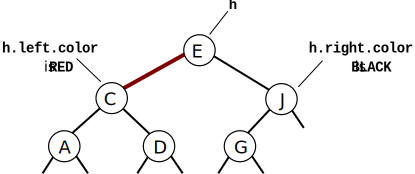
\includegraphics[scale=0.4]{{./figures/red_black_bst4}.pdf}}
\end{center}
\end{minipage}
\end{frame}

\section{Elementary Red-black BST Operations}
\begin{frame}[fragile]
\pause

Elementary red-black BST operations (left/right rotation and color flip) maintain symmetric order and perfect black balance

\pause
\bigskip

Left rotation: orient a (temporarily) right-leaning red link to lean left
\begin{center}
\pause
\visible<4->{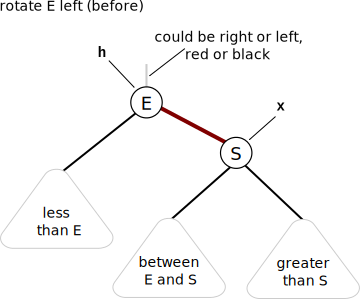
\includegraphics[scale=0.4]{{./figures/red_black_bst5}.pdf}}\hspace{10mm}
\pause
\visible<5->{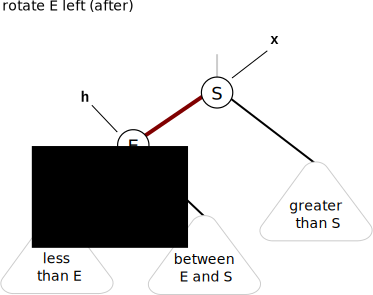
\includegraphics[scale=0.4]{{./figures/red_black_bst6}.pdf}}
\end{center}

\pause
\bigskip

Implementation of left rotation
\begin{lstlisting}[language=Java,style=focusin]
private Node rotateLeft(Node h) {
    Node x = h.right;
    h.right = x.left;
    x.left = h;
    x.color = x.left.color;
    x.left.color = RED;
    x.N = h.N;
    h.N = size(h.left) + size(h.right) + 1;
    return x;
}
\end{lstlisting}
\end{frame}

\begin{frame}[fragile]
\pause

Right rotation: orient a left-leaning red link to (temporarily) lean right
\begin{center}
\pause
\visible<3->{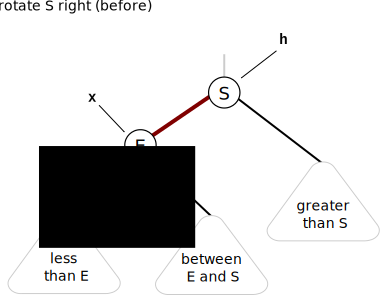
\includegraphics[scale=0.4]{{./figures/red_black_bst7}.pdf}}\hspace{10mm}
\pause
\visible<4->{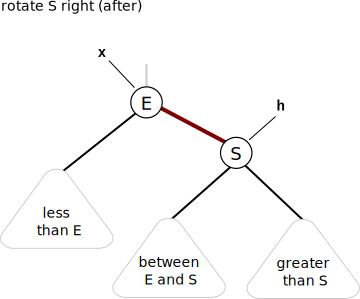
\includegraphics[scale=0.4]{{./figures/red_black_bst8}.pdf}}
\end{center}

\pause
\bigskip

Implementation of right rotation

\begin{lstlisting}[language=Java,style=focusin]
private Node rotateRight(Node h) {
    Node x = h.left;
    h.left = x.right;
    x.right = h;
    x.color = x.right.color;
    x.right.color = RED;
    x.N = h.N;
    h.N = size(h.left) + size(h.right) + 1;
    return x;
}
\end{lstlisting}
\end{frame}

\begin{frame}[fragile]
\pause

Color flip: recolor to split a (temporary) 4-node
\begin{center}
\pause
\visible<3->{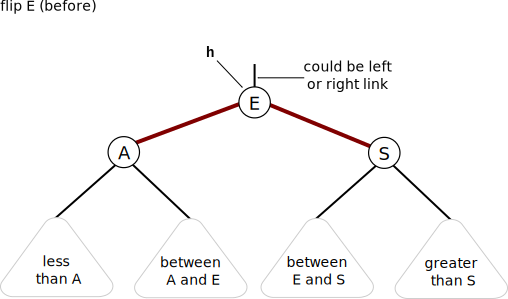
\includegraphics[scale=0.35]{{./figures/red_black_bst9}.pdf}}\hspace{5mm}
\pause
\visible<4->{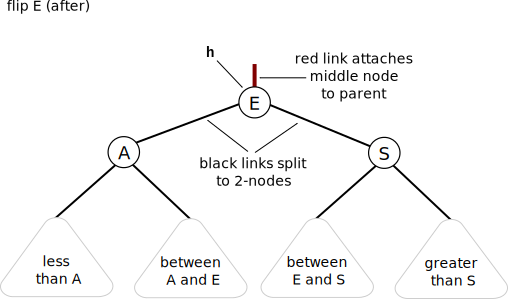
\includegraphics[scale=0.35]{{./figures/red_black_bst10}.pdf}}
\end{center}

\pause
\bigskip

Implementation of color flip

\begin{lstlisting}[language=Java,style=focusin]
private void flipColors(Node h) {
    h.color = !h.color;
    h.left.color = !h.left.color;
    h.right.color = !h.right.color;
}
\end{lstlisting}
\end{frame}

\section{Implementation of the Ordered Symbol Table API Using a Red-Black BST}
\begin{frame}[fragile]
\pause

Most operations are the same as for BST-based implementation --- ignore color

\pause
\bigskip

Insertion: the basic strategy is to maintain 1-1 correspondence with 2-3 trees, using the elementary red-black BST operations (left/right rotation and color flip) to maintain symmetric order and perfect balance, but not necessarily color invariants

\pause
\bigskip

Case 1 (insert into a 2-node at the bottom): do standard BST insert; color new link red; if new red link is a right link, rotate left

\begin{center}
\visible<4->{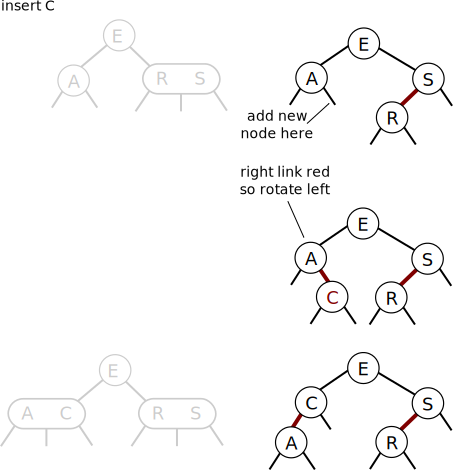
\includegraphics[scale=0.4]{{./figures/red_black_bst11}.pdf}}
\end{center}
\end{frame}

\begin{frame}[fragile]
\pause

Case 2 (insert into a 3-node at the bottom): do standard BST insert; color new link red; rotate to balance the 4-node (if needed); flip colors to pass red link up one level; rotate to make lean left (if needed); repeat case 1 or case 2 up the tree (if needed)

\begin{center}
\visible<2->{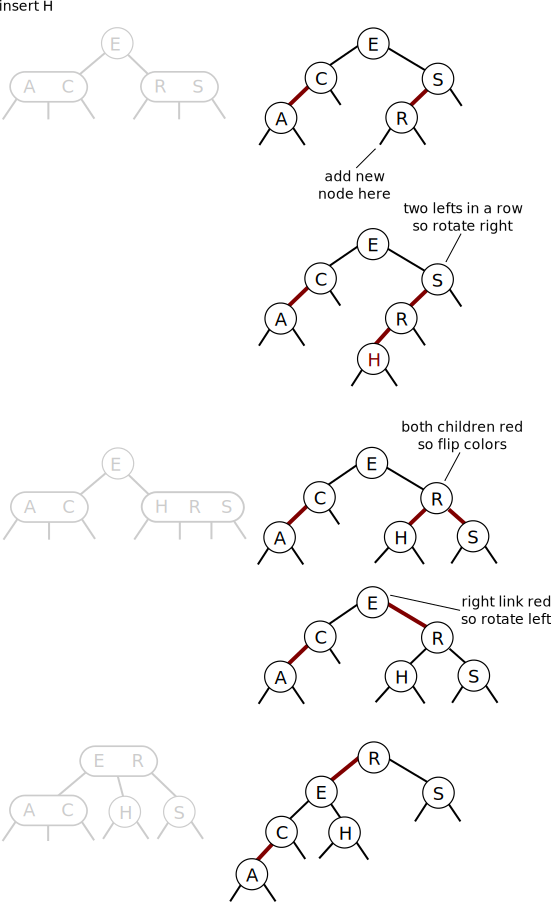
\includegraphics[scale=0.3]{{./figures/red_black_bst12}.pdf}}
\end{center}
\end{frame}

\begin{frame}[fragile]
\pause

\begin{minipage}{150pt}
Implementation (same code for all cases)
\begin{itemize}
\pause
\item Right child red, left child black: rotate left
\pause
\item Left child, left-left grandchild red: rotate right
\pause
\item Both children red: flip colors
\end{itemize}
\end{minipage}%
\begin{minipage}{100pt}
\begin{center}
\visible<6->{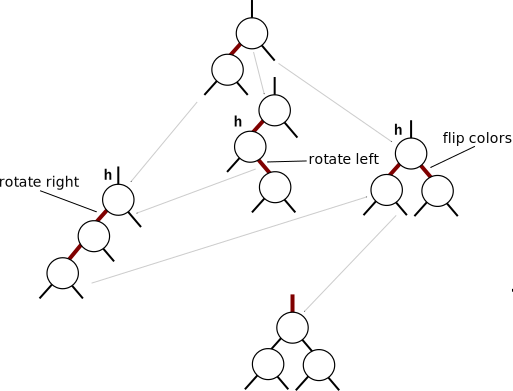
\includegraphics[scale=0.4]{{./figures/red_black_bst13}.pdf}}
\end{center}
\end{minipage}
\end{frame}

\begin{frame}[fragile]
\pause

\begin{lstlisting}[language=Java,style=focusin]
package edu.princeton.cs.algs4;

import java.util.NoSuchElementException;

public class RedBlackBST<Key extends Comparable<Key>, Value> {
    private Node root;

    public void put(Key key, Value val) {
        root = put(root, key, val); root.color = BLACK;
    }

    private Node put(Node h, Key key, Value val) { 
        if (h == null) { return new Node(key, val, RED, 1); }
        int cmp = key.compareTo(h.key);
        if      (cmp < 0) { h.left  = put(h.left,  key, val); }
        else if (cmp > 0) { h.right = put(h.right, key, val); }
        else              { h.val   = val; }
        if (isRed(h.right) && !isRed(h.left))      { h = rotateLeft(h); }
        if (isRed(h.left)  &&  isRed(h.left.left)) { h = rotateRight(h); }
        if (isRed(h.left)  &&  isRed(h.right))     { flipColors(h); }
        h.N = size(h.left) + size(h.right) + 1;
        return h;
    }
}
\end{lstlisting}
\end{frame}

\begin{frame}[fragile]
\pause

Deletion: see exercises 3.3.39 -- 3.3.41

\pause
\bigskip

The average length of a path from the root to a node in a red-black BST with $N$ nodes is $\sim \lg N$

\pause
\bigskip

Typical red-black BST built from random keys (null links omitted)
\begin{center}
\visible<4->{\includegraphics[scale=0.35]{{./figures/red_black_bst14}.png}}
\end{center}

\pause
\bigskip

Red-black BST built from ascending keys (null links omitted)
\begin{center}
\visible<5->{\includegraphics[scale=0.35]{{./figures/red_black_bst15}.png}}
\end{center}
\end{frame}

\section{Performance Characteristics}
\begin{frame}[fragile]
\pause

Symbol table operations summary

\begin{center}
\begin{tabular}{ccc}
operation & BST & red-black BST \\ \hline
search & $h^\dagger$ & $\lg N$ \\
insert & $h$ & $\lg N$ \\
delete & $\sqrt{N}^{\dagger\dagger}$ & $\lg N$ \\
min/max & $h$ & $\lg N$ \\
floor/ceiling & $h$ & $\lg N$ \\
rank & $h$ & $\lg N$ \\
select & $h$ & $\lg N$ \\
ordered iteration & $N$ & $N$ 
\end{tabular}

\bigskip

\tiny $\dagger$ $h$ is the height of BST, proportional to $\lg N$ if keys inserted in random order

$\dagger\dagger$ $\sqrt{N}$ other operations also become $\sqrt{N}$ if deletions are allowed
\end{center} 
\end{frame}
\end{document}
